\section{Проектирования программного средства}


\subsection{Общая информация}

Для реализации системы будет использован язык программирования
C\# 8. Он предоставляет высокую производительность и
эффективность разработки, что особенно важно для системы, которая должна
обрабатывать большое количество запросов на поиск и выдачу ответов. Проект
будет разрабатываться на операционной системе linux, которая является
одной из популярных операционных систем.

В качестве СУБД будет использована SQLite3, а также для работы с ней 
будет задействована технология с поддержкой ORM (object-relational mapping - отображения данных на реальные объекты)
Entity Framework Core.

Для обработки пользовательских REST (передача состояния представления) запросов будет использована платформа ASP.NET,
а также уведомление пользоватей пользователей об изменном состоянии системы аукциона в режиме реального времени
будет проходить с применением библиотеки SignalR, используя WebSockets, Server-Sent Events и Long Polling. 

Для удобства разработки будет задействована система контроля версий Git 
и платформа GitHub для хостинга репозитория. 
Это позволит легко отслеживать изменения в коде и управлять различными версиями. 
Кроме того, будет использоваться редактор кода Visual Studio Code (Vs Code), 
который обладает множеством полезных функций, 
таких как автодополнение кода, отладка и интеграция с Git, 
что создаст комфортную среду разработки и повысит производительность.

Для тестирования приложения будет использован программное средство Postman. 
Postman - это популярный инструмент для тестирования API, который позволяет отправлять запросы к серверу и получать ответы. 
Он также может быть использован для документирования API и создания запросов.

\subsection{Разработка функциональности программного средства}

При анализе требований для реализации программного продукта для тестирования была построена use-case диаграмма, 
которая отображает взаимодействие между пользователем и приложением. 
На рисунке 2.1, представленном ниже, отображены основные возможности использования приложения.

\newpage
\begin{figure}[h]
\centering
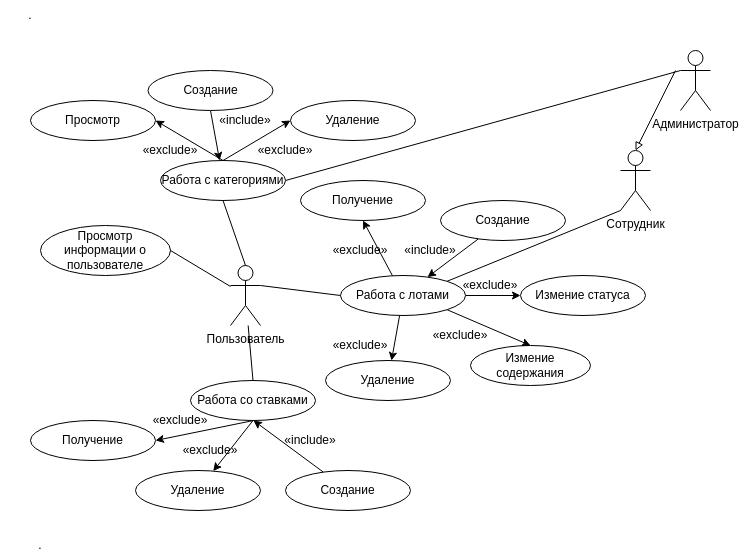
\includegraphics[scale=0.5]{usecase.drawio.png}
\caption{Use-case диаграмма приложения}
\end{figure}

Таким образом рассмотрены возможности использования от лица обычного пользователя, от лица администратора и сотрудника.

\subsection{Архитектура программного средства}

В качестве архитектуры приложения была выбрана трёхуровневая архитектура.
В приложении можно выделить следующие слои:

– слой инфраструктуры – обеспечивает доступ к данным, 
реализует паттерны репозиторий и Unit of Work, 
содержит реализацию абстракции репозитория и классов для работы непосредственно с базой данных. 
Вся работа с базой данных происходит в репозиториях, 
которые объединены классов Unit of Work, организующим всю работу с базой данных;  

– слой приложения – полностью независимый слой, который определяет модели и абстракции для работы с базой данных, а также содержит 
бизнес-логику системы аукциона.

– слой представления – содержит реализованный с использованием платформы
ASP.NET Core веб-интерфейс приложения. При помощи библиотеки SignalR реализует
обмен сообщениями об изменном состоянии системы аукциона между клиентом и сервером.
Также данный слой реализует систему авторизации и аутентификации пользователей.

% Также при разработке приложения использовались следующие концепции проектирования архитектуры:

% – Репозиторий – это архитектурный паттерн, который предлагает абстракцию слоя доступа к данным. 
% Его цель – скрыть детали реализации базы данных или другого хранилища данных от остальной части приложения;

% – Unit Of Work – это архитектурный паттерн, 
% который помогает упростить работу с различными репозиториями 
% и обеспечивает единое управление изменениями в базе данных в рамках одной логической транзакции;

% – Внедрение зависимостей – процесс предоставления внешней зависимости программному компоненту. 
% Является специфичной формой «инверсии управления» (Inversion of control, IoC), 
% когда она применяется к управлению зависимостями. 
% В полном соответствии с принципом единственной ответсвенности объект отдаёт заботу 
% о построении требуемых ему зависимостей внешнему, специально предназначенному для этого общему механизму;

% – Data Transfer Object (DTO) – шаблон проектирования, 
% используемый для определения формата, 
% в котором данные передаются между клиентским и серверным приложениями.